\chapter{Introduzione ai Boosted Decision Tree}

In questa tesi l'analisi dati per la selezione del mesone $D^{*+}$ \`e stata svolta utilizzando algoritmi di machine learning (apprendimento artificaile).\footnote{machine larning: meccanismo che permette ad una macchina intelligente di migliorare le proprie prestazioni nel tempo. \cite{sitoMachineLearning}} Questo per confrontare i risultati ottenuto con questo metodo con quelli dell'analisi standard di ALICE. In questo capitolo si illustrano pertanto le caratteristiche principali dell'algoritmo di machine learning utilizzato.  

\section{Analisi Multivariata e Problemi di Selezione} \label{AnalisiMulti}
Il machine learning consiste nello sviluppo di algoritmi che possono imparare dai dati e in base ad essi prendere decisioni o fare previsioni. Il machine learning può essere di tipo supervisionato o non supervisionato. Nel primo caso si utilizzano degli esempi per addestrare l'algoritmo di cui si fornisce anche la "risposta". In questo modo vi è una sorta di feedback su cui si basa l'addestramento. Nel caso non supervisionato, al contrario, vengono forniti solo dei dati e sarà l'algoritmo stesso a decidere indipendentemente come classificarli. L' \textit{analisi multivariata}  appartiene al caso del machine learning supervisionato. Prevede, infatti, che tutte le variabili vengano combinate (in base al metodo scelto) in un'unica variabile finale, chiamata \textit{classifier output}, che fornisce il metodo di valutazione finale.
\\In questa tesi si affronta un \textit{problema di selezione}, ovvero si cerca un segnale raro in un insieme composto principalmente da eventi di fondo, per cui il rapporto segnale su fondo \`e basso.
Per l'analisi svolta in questa tesi \`e stato utilizzato il "TMVA" (Tool for MultiVariate Analysis), che \`e uno strumento incluso in Root che implementa diversi metodi di analisi multivariata. L'analisi effettuata si struttura in due fasi principali:
    \begin{itemize}
        \item Training: in questa fase l'algoritmo analizza dati di cui conosce gi\`a il tipo e li utilizza per apprendere quali sono le caratteristiche dei vari tipi di dati;
        \item Applicazione: nella fase di applicazione viene utilizzato quanto appreso dalla macchina nella fase di training per selezionare e dividere dati di cui non si conosce il tipo.
    \end{itemize}
    
\section{Boosted Decision Tree} \label{BDT}

    \subsection{Alberi decisionali}
    Un \textit{albero decisionale} (decision tree) è una struttura che classifica i dati mediante scelte di tipo binario. Se ne riporta un esempio base in figura \ref{fig:BDT}. Ogni scelta è basata su una selezione su una singola variabile. %Ogni scelta è basata su un taglio su una singola variabile.
    Ogni ramo creato viene poi nuovamente diviso in due in base al taglio su un'altra variabile. I gruppi di dati creati alla fine dell'albero sono chiamati foglie. Queste vengono selezionate come segnale o background in base alla classe cui appartiene la maggior parte degli eventi. 
    
    \begin{figure}[htbp]
        \centering
        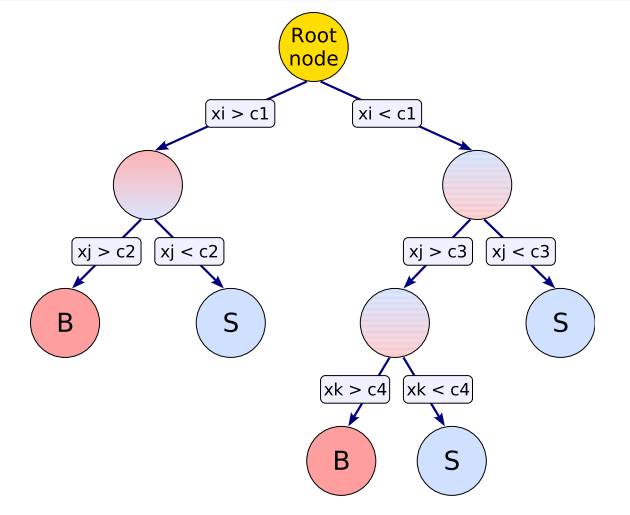
\includegraphics[width=0.5\linewidth]{TMVA/BDT1.PNG}
        \caption{ Esempio di schema di un decision tree}
        \label{fig:BDT}
    \end{figure}
    
    Un vantaggio dei decision tree è che sono facilmente visualizzabili ed è altrettanto semplice ricondursi al significato fisico dei tagli operati. Inoltre sono perlopiù insensibili alla presenza di variabili poco discriminanti (cosa che non accade, invece, per molte altre tecniche di analisi multivariata). Lo svantaggio principale è che sono fortemente sensibili alle fluttuazioni statistiche dei dati utilizzati per il training. Questo problema viene risolto con il "boosting" di cui si parla nella sezione  \ref{Boosting}.
    \\Per poter creare il decision tree \`e necessario un set di dati per il \textit{training}, ovvero dei dati di cui si consce già se siano segnale o fondo. La prima divisione dei dati, chiamata root node, viene scelta individuando la variabile e il suo relativo taglio che meglio divide i dati tra segnale e background. L'indice di separazione utilizzato in questa tesi è quello di Gini \footnote{L'indice di Gini è definito come: $p (1-p)$, dove $p$ è la purezza del segnale, che è il rapporto tra il numero di eventi segnale e il numero di eventi totale}. A questo punto si considera singolarmente ognuno dei due rami e si sceglie il taglio sulla variabile che massimizza l'aumento dell'indice di separazione. Si continua così finchè non viene raggiunto uno dei criteri di stop,  a questo punto la struttura dell'albero è formata ed è possibile verificare in che modo sono stati divisi i dati tra segnale e background. 
    \\Infine è necessario fare un controllo per l'\textit{overtraining}, ovvero la possibilità che il decision tree si sia sensibilizzato eccessivamente al set di dati utilizzati nella fase di training e non sia più descrittivo del fenomeno fisico nella sua generalità. Per fare ciò si utilizzano dei dati generati da simulazione, che però non sono stati utilizzati nella fase di training e si controlla che la risposta del decision tree sui dati del training e su questi nuovi dati (detti dati del testing) sia simile.\cite{TMVAGuide} 
 
    \subsection{Boosting} \label{Boosting}
    Per migliorare le performance dell'algoritmo di amchine learning \`e utile utilizzare il meccanismo del \textit{boosting}. Questo viene utilizzato nel caso dei decision tree per renderli più stabili rispetto alle fluttuazioni statistiche del set di dati del training e per migliorarne la capacit\`a di selezionare i dati. Per fare ciò l'algoritmo ripete automaticamente il training pi\`u volte utilizzando lo stesso set di dati e ad ogni ripetizione d\`a pesi diversi ai dati.
    \\L'algoritmo di boosting utilizzato in questa tesi è l'\textit{Adaptive Boosting} (AdaBoost). In questo caso i dati che sono stati classificati erroneamente nel precedente decision tree vengono ripesati con un fattore $\alpha$, che è calcolato come 
        \begin{equation}
            \alpha = \frac{1 - err}{err}
        \end{equation}
    Dove $err$ è il rate di eventi classificati erroneamente. 
    \\Si viene a creare una foresta di decision tree da cui si deriva il responso finale per la selezione degli eventi. Gli algoritmi di boosting funzionano meglio se si utilizzano alberi piccoli, ovvero con pochi livelli di diramazione.
    Utilizzando questa tecnica, pertanto, si riesce a rendere l'algoritmo più stabile ed efficiente ma d'altra parte si perde il senso fisico della selezione tra segnale e fondo. 
    
    
    
    
